En esta sección detallaremos el Modelo Conceptual creado para el TP. La representación del mismo consiste en un Diagrama
de entidad relación.

\begin{figure}[H]
  \centering
    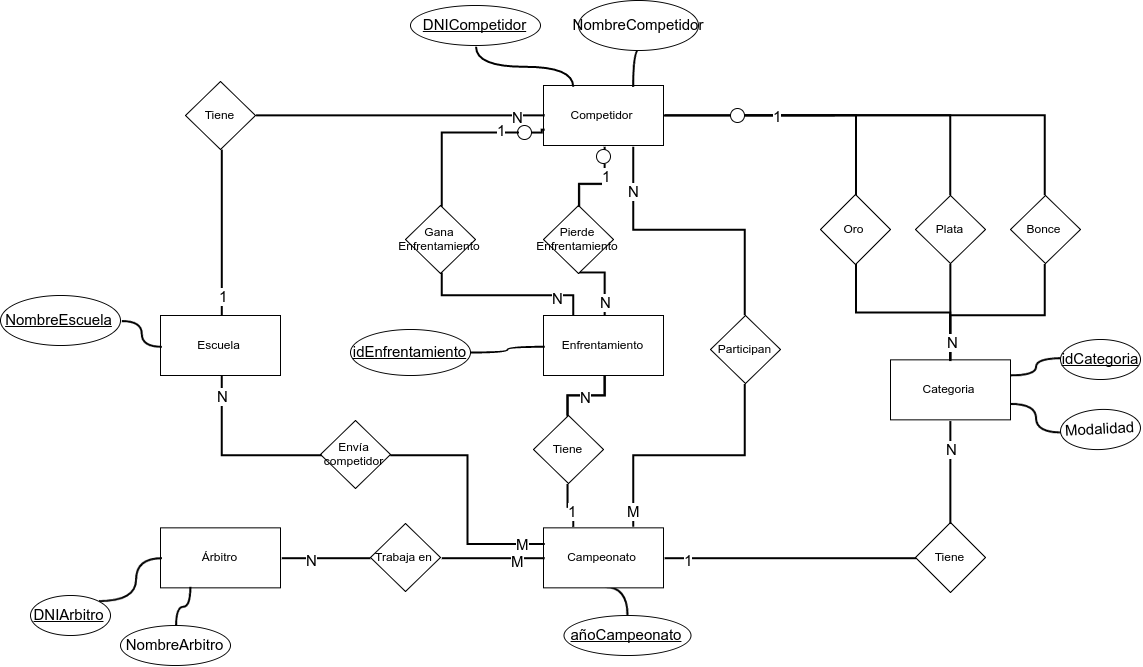
\includegraphics[scale=0.4]{imagenes/DER.png}
  \caption{Diagrama entidad relación}
\end{figure}

A continuación detallaremos las distintas entidades y sus relaciones.\\

Los árbitros poseen un DNI, que sirve como identificador y clave primaria, y un nombre. Cada árbitro participo históricamente
en muchos campeonatos.\\

Las escuelas se identifican con un nombre y envían a sus competidores a los distintos campeonatos. Cada escuela conoce los competidores
que posee y los campeonatos a los que mando competidores.\\

Los campeonatos poseen un año, usado como clave primaria. Cada campeonato tiene muchas categorías. Cada una de estas se
traduce en enfrentamientos entre dos competidores. Por lo tanto, el campeonato tiene muchos enfrentamientos. Además
el campeonato registra a los competidores que participan de los enfrentamientos. Como los competidores provienen de
diversas escuelas.\\

Cada categoría es identificada con un idCategoría. Además cada una tiene una modalidad, las cuales pueden ser
Combate, Formas o Rotura. Existen tres tipos de medallas por categoría: oro, plata y bronce. Estas medallas son ganadas
por los competidores de los enfrentamientos de esa categoría.\\

Los competidores tienen como clave primaria su DNI y poseen un nombre. Los competidores representan a una sola escuela en
los campeonatos. A la vez, pueden haber participado en varios campeonatos. Dado que cada competidor puede participar
de varias categorías por campeonato, también puede haber resultado victorioso o derrotado en varios enfrentamientos por
cada campeonato al que participo. También puede haber ganado medallas, de cualquiera de los tres tipo, en más de una categoría.
O podría no haber ganado ninguna.\\

Los enfrentamientos se realizan para un campeonato específico y en él participan dos competidores distintos. Uno de estos
es el ganador del enfrentamiento y otro el perdedor.
